\documentclass[12pt]{article}

%packages
%\usepackage{latexsym}
\usepackage{graphicx}
\usepackage{color}
\usepackage{amsmath}
\usepackage{dsfont}
\usepackage{placeins}
\usepackage{amssymb}
\usepackage{wasysym}
\usepackage{abstract}
\usepackage{hyperref}
\usepackage{etoolbox}
\usepackage{datetime}
\usepackage{xcolor}
\usepackage{alphalph}
\settimeformat{ampmtime}

%\usepackage{pstricks,pst-node,pst-tree}

%\usepackage{algpseudocode}
%\usepackage{amsthm}
%\usepackage{hyperref}
%\usepackage{mathrsfs}
%\usepackage{amsfonts}
%\usepackage{bbding}
%\usepackage{listings}
%\usepackage{appendix}
\usepackage[margin=1in]{geometry}
%\geometry{papersize={8.5in,11in},total={6.5in,9in}}
%\usepackage{cancel}
%\usepackage{algorithmic, algorithm}

\makeatletter
\def\maxwidth{ %
  \ifdim\Gin@nat@width>\linewidth
    \linewidth
  \else
    \Gin@nat@width
  \fi
}
\makeatother

\definecolor{fgcolor}{rgb}{0.345, 0.345, 0.345}
\newcommand{\hlnum}[1]{\textcolor[rgb]{0.686,0.059,0.569}{#1}}%
\newcommand{\hlstr}[1]{\textcolor[rgb]{0.192,0.494,0.8}{#1}}%
\newcommand{\hlcom}[1]{\textcolor[rgb]{0.678,0.584,0.686}{\textit{#1}}}%
\newcommand{\hlopt}[1]{\textcolor[rgb]{0,0,0}{#1}}%
\newcommand{\hlstd}[1]{\textcolor[rgb]{0.345,0.345,0.345}{#1}}%
\newcommand{\hlkwa}[1]{\textcolor[rgb]{0.161,0.373,0.58}{\textbf{#1}}}%
\newcommand{\hlkwb}[1]{\textcolor[rgb]{0.69,0.353,0.396}{#1}}%
\newcommand{\hlkwc}[1]{\textcolor[rgb]{0.333,0.667,0.333}{#1}}%
\newcommand{\hlkwd}[1]{\textcolor[rgb]{0.737,0.353,0.396}{\textbf{#1}}}%

\usepackage{framed}
\makeatletter
\newenvironment{kframe}{%
 \def\at@end@of@kframe{}%
 \ifinner\ifhmode%
  \def\at@end@of@kframe{\end{minipage}}%
  \begin{minipage}{\columnwidth}%
 \fi\fi%
 \def\FrameCommand##1{\hskip\@totalleftmargin \hskip-\fboxsep
 \colorbox{shadecolor}{##1}\hskip-\fboxsep
     % There is no \\@totalrightmargin, so:
     \hskip-\linewidth \hskip-\@totalleftmargin \hskip\columnwidth}%
 \MakeFramed {\advance\hsize-\width
   \@totalleftmargin\z@ \linewidth\hsize
   \@setminipage}}%
 {\par\unskip\endMakeFramed%
 \at@end@of@kframe}
\makeatother

\definecolor{shadecolor}{rgb}{.77, .77, .77}
\definecolor{messagecolor}{rgb}{0, 0, 0}
\definecolor{warningcolor}{rgb}{1, 0, 1}
\definecolor{errorcolor}{rgb}{1, 0, 0}
\newenvironment{knitrout}{}{} % an empty environment to be redefined in TeX

\usepackage{alltt}
\usepackage[T1]{fontenc}

\newcommand{\qu}[1]{``#1''}
\newcounter{probnum}
\setcounter{probnum}{1}

%create definition to allow local margin changes
\def\changemargin#1#2{\list{}{\rightmargin#2\leftmargin#1}\item[]}
\let\endchangemargin=\endlist 

%allow equations to span multiple pages
\allowdisplaybreaks

%define colors and color typesetting conveniences
\definecolor{gray}{rgb}{0.5,0.5,0.5}
\definecolor{black}{rgb}{0,0,0}
\definecolor{white}{rgb}{1,1,1}
\definecolor{blue}{rgb}{0.5,0.5,1}
\newcommand{\inblue}[1]{\color{blue}#1 \color{black}}
\definecolor{green}{rgb}{0.133,0.545,0.133}
\newcommand{\ingreen}[1]{\color{green}#1 \color{black}}
\definecolor{yellow}{rgb}{1,1,0}
\newcommand{\inyellow}[1]{\color{yellow}#1 \color{black}}
\definecolor{orange}{rgb}{0.9,0.649,0}
\newcommand{\inorange}[1]{\color{orange}#1 \color{black}}
\definecolor{red}{rgb}{1,0.133,0.133}
\newcommand{\inred}[1]{\color{red}#1 \color{black}}
\definecolor{purple}{rgb}{0.58,0,0.827}
\newcommand{\inpurple}[1]{\color{purple}#1 \color{black}}
\definecolor{backgcode}{rgb}{0.97,0.97,0.8}
\definecolor{Brown}{cmyk}{0,0.81,1,0.60}
\definecolor{OliveGreen}{cmyk}{0.64,0,0.95,0.40}
\definecolor{CadetBlue}{cmyk}{0.62,0.57,0.23,0}

%define new math operators
\DeclareMathOperator*{\argmax}{arg\,max~}
\DeclareMathOperator*{\argmin}{arg\,min~}
\DeclareMathOperator*{\argsup}{arg\,sup~}
\DeclareMathOperator*{\arginf}{arg\,inf~}
\DeclareMathOperator*{\convolution}{\text{\Huge{$\ast$}}}
\newcommand{\infconv}[2]{\convolution^\infty_{#1 = 1} #2}
%true functions

%%%% GENERAL SHORTCUTS

%shortcuts for pure typesetting conveniences
\newcommand{\bv}[1]{\boldsymbol{#1}}

%shortcuts for compound constants
\newcommand{\BetaDistrConst}{\dfrac{\Gamma(\alpha + \beta)}{\Gamma(\alpha)\Gamma(\beta)}}
\newcommand{\NormDistrConst}{\dfrac{1}{\sqrt{2\pi\sigma^2}}}

%shortcuts for conventional symbols
\newcommand{\tsq}{\tau^2}
\newcommand{\tsqh}{\hat{\tau}^2}
\newcommand{\sigsq}{\sigma^2}
\newcommand{\sigsqsq}{\parens{\sigma^2}^2}
\newcommand{\sigsqovern}{\dfrac{\sigsq}{n}}
\newcommand{\tausq}{\tau^2}
\newcommand{\tausqalpha}{\tau^2_\alpha}
\newcommand{\tausqbeta}{\tau^2_\beta}
\newcommand{\tausqsigma}{\tau^2_\sigma}
\newcommand{\betasq}{\beta^2}
\newcommand{\sigsqvec}{\bv{\sigma}^2}
\newcommand{\sigsqhat}{\hat{\sigma}^2}
\newcommand{\sigsqhatmlebayes}{\sigsqhat_{\text{Bayes, MLE}}}
\newcommand{\sigsqhatmle}[1]{\sigsqhat_{#1, \text{MLE}}}
\newcommand{\bSigma}{\bv{\Sigma}}
\newcommand{\bSigmainv}{\bSigma^{-1}}
\newcommand{\thetavec}{\bv{\theta}}
\newcommand{\thetahat}{\hat{\theta}}
\newcommand{\thetahatmle}{\hat{\theta}_{\mathrm{MLE}}}
\newcommand{\thetavechatmle}{\hat{\thetavec}_{\mathrm{MLE}}}
\newcommand{\muhat}{\hat{\mu}}
\newcommand{\musq}{\mu^2}
\newcommand{\muvec}{\bv{\mu}}
\newcommand{\muhatmle}{\muhat_{\text{MLE}}}
\newcommand{\lambdahat}{\hat{\lambda}}
\newcommand{\lambdahatmle}{\lambdahat_{\text{MLE}}}
\newcommand{\etavec}{\bv{\eta}}
\newcommand{\alphavec}{\bv{\alpha}}
\newcommand{\minimaxdec}{\delta^*_{\mathrm{mm}}}
\newcommand{\ybar}{\bar{y}}
\newcommand{\xbar}{\bar{x}}
\newcommand{\Xbar}{\bar{X}}
\newcommand{\phat}{\hat{p}}
\newcommand{\Phat}{\hat{P}}
\newcommand{\Zbar}{\bar{Z}}
\newcommand{\iid}{~{\buildrel iid \over \sim}~}
\newcommand{\inddist}{~{\buildrel ind \over \sim}~}
\newcommand{\approxdist}{~{\buildrel approx \over \sim}~}
\newcommand{\equalsindist}{~{\buildrel d \over =}~}
\newcommand{\loglik}[1]{\ell\parens{#1}}
\newcommand{\thetahatkminone}{\thetahat^{(k-1)}}
\newcommand{\thetahatkplusone}{\thetahat^{(k+1)}}
\newcommand{\thetahatk}{\thetahat^{(k)}}
\newcommand{\half}{\frac{1}{2}}
\newcommand{\third}{\frac{1}{3}}
\newcommand{\twothirds}{\frac{2}{3}}
\newcommand{\fourth}{\frac{1}{4}}
\newcommand{\fifth}{\frac{1}{5}}
\newcommand{\sixth}{\frac{1}{6}}

%shortcuts for vector and matrix notation
\newcommand{\A}{\bv{A}}
\newcommand{\At}{\A^T}
\newcommand{\Ainv}{\inverse{\A}}
\newcommand{\B}{\bv{B}}
\newcommand{\K}{\bv{K}}
\newcommand{\Kt}{\K^T}
\newcommand{\Kinv}{\inverse{K}}
\newcommand{\Kinvt}{(\Kinv)^T}
\newcommand{\M}{\bv{M}}
\newcommand{\Bt}{\B^T}
\newcommand{\Q}{\bv{Q}}
\newcommand{\Qt}{\Q^T}
\newcommand{\R}{\bv{R}}
\newcommand{\Rt}{\R^T}
\newcommand{\Z}{\bv{Z}}
\newcommand{\X}{\bv{X}}
\newcommand{\Xsub}{\X_{\text{(sub)}}}
\newcommand{\Xsubadj}{\X_{\text{(sub,adj)}}}
\newcommand{\I}{\bv{I}}
\newcommand{\Y}{\bv{Y}}
\newcommand{\sigsqI}{\sigsq\I}
\renewcommand{\P}{\bv{P}}
\newcommand{\Psub}{\P_{\text{(sub)}}}
\newcommand{\Pt}{\P^T}
\newcommand{\Pii}{P_{ii}}
\newcommand{\Pij}{P_{ij}}
\newcommand{\IminP}{(\I-\P)}
\newcommand{\Xt}{\bv{X}^T}
\newcommand{\XtX}{\Xt\X}
\newcommand{\XtXinv}{\parens{\Xt\X}^{-1}}
\newcommand{\XtXinvXt}{\XtXinv\Xt}
\newcommand{\XXtXinvXt}{\X\XtXinvXt}
\newcommand{\x}{\bv{x}}
\newcommand{\onevec}{\bv{1}}
\newcommand{\oneton}{1, \ldots, n}
\newcommand{\yoneton}{y_1, \ldots, y_n}
\newcommand{\yonetonorder}{y_{(1)}, \ldots, y_{(n)}}
\newcommand{\Yoneton}{Y_1, \ldots, Y_n}
\newcommand{\iinoneton}{i \in \braces{\oneton}}
\newcommand{\onetom}{1, \ldots, m}
\newcommand{\jinonetom}{j \in \braces{\onetom}}
\newcommand{\xoneton}{x_1, \ldots, x_n}
\newcommand{\Xoneton}{X_1, \ldots, X_n}
\newcommand{\xt}{\x^T}
\newcommand{\y}{\bv{y}}
\newcommand{\yt}{\y^T}
\renewcommand{\c}{\bv{c}}
\newcommand{\ct}{\c^T}
\newcommand{\tstar}{\bv{t}^*}
\renewcommand{\u}{\bv{u}}
\renewcommand{\v}{\bv{v}}
\renewcommand{\a}{\bv{a}}
\newcommand{\s}{\bv{s}}
\newcommand{\yadj}{\y_{\text{(adj)}}}
\newcommand{\xjadj}{\x_{j\text{(adj)}}}
\newcommand{\xjadjM}{\x_{j \perp M}}
\newcommand{\yhat}{\hat{\y}}
\newcommand{\yhatsub}{\yhat_{\text{(sub)}}}
\newcommand{\yhatstar}{\yhat^*}
\newcommand{\yhatstarnew}{\yhatstar_{\text{new}}}
\newcommand{\z}{\bv{z}}
\newcommand{\zt}{\z^T}
\newcommand{\bb}{\bv{b}}
\newcommand{\bbt}{\bb^T}
\newcommand{\bbeta}{\bv{\beta}}
\newcommand{\beps}{\bv{\epsilon}}
\newcommand{\bepst}{\beps^T}
\newcommand{\e}{\bv{e}}
\newcommand{\Mofy}{\M(\y)}
\newcommand{\KofAlpha}{K(\alpha)}
\newcommand{\ellset}{\mathcal{L}}
\newcommand{\oneminalph}{1-\alpha}
\newcommand{\SSE}{\text{SSE}}
\newcommand{\SSEsub}{\text{SSE}_{\text{(sub)}}}
\newcommand{\MSE}{\text{MSE}}
\newcommand{\RMSE}{\text{RMSE}}
\newcommand{\SSR}{\text{SSR}}
\newcommand{\SST}{\text{SST}}
\newcommand{\JSest}{\delta_{\text{JS}}(\x)}
\newcommand{\Bayesest}{\delta_{\text{Bayes}}(\x)}
\newcommand{\EmpBayesest}{\delta_{\text{EmpBayes}}(\x)}
\newcommand{\BLUPest}{\delta_{\text{BLUP}}}
\newcommand{\MLEest}[1]{\hat{#1}_{\text{MLE}}}

%shortcuts for Linear Algebra stuff (i.e. vectors and matrices)
\newcommand{\twovec}[2]{\bracks{\begin{array}{c} #1 \\ #2 \end{array}}}
\newcommand{\threevec}[3]{\bracks{\begin{array}{c} #1 \\ #2 \\ #3 \end{array}}}
\newcommand{\fivevec}[5]{\bracks{\begin{array}{c} #1 \\ #2 \\ #3 \\ #4 \\ #5 \end{array}}}
\newcommand{\twobytwomat}[4]{\bracks{\begin{array}{cc} #1 & #2 \\ #3 & #4 \end{array}}}
\newcommand{\threebytwomat}[6]{\bracks{\begin{array}{cc} #1 & #2 \\ #3 & #4 \\ #5 & #6 \end{array}}}

%shortcuts for conventional compound symbols
\newcommand{\thetainthetas}{\theta \in \Theta}
\newcommand{\reals}{\mathbb{R}}
\newcommand{\complexes}{\mathbb{C}}
\newcommand{\rationals}{\mathbb{Q}}
\newcommand{\integers}{\mathbb{Z}}
\newcommand{\naturals}{\mathbb{N}}
\newcommand{\forallninN}{~~\forall n \in \naturals}
\newcommand{\forallxinN}[1]{~~\forall #1 \in \reals}
\newcommand{\matrixdims}[2]{\in \reals^{\,#1 \times #2}}
\newcommand{\inRn}[1]{\in \reals^{\,#1}}
\newcommand{\mathimplies}{\quad\Rightarrow\quad}
\newcommand{\mathlogicequiv}{\quad\Leftrightarrow\quad}
\newcommand{\eqncomment}[1]{\quad \text{(#1)}}
\newcommand{\limitn}{\lim_{n \rightarrow \infty}}
\newcommand{\limitN}{\lim_{N \rightarrow \infty}}
\newcommand{\limitd}{\lim_{d \rightarrow \infty}}
\newcommand{\limitt}{\lim_{t \rightarrow \infty}}
\newcommand{\limitsupn}{\limsup_{n \rightarrow \infty}~}
\newcommand{\limitinfn}{\liminf_{n \rightarrow \infty}~}
\newcommand{\limitk}{\lim_{k \rightarrow \infty}}
\newcommand{\limsupn}{\limsup_{n \rightarrow \infty}}
\newcommand{\limsupk}{\limsup_{k \rightarrow \infty}}
\newcommand{\floor}[1]{\left\lfloor #1 \right\rfloor}
\newcommand{\ceil}[1]{\left\lceil #1 \right\rceil}

%shortcuts for environments
\newcommand{\beqn}{\vspace{-0.25cm}\begin{eqnarray*}}
\newcommand{\eeqn}{\end{eqnarray*}}
\newcommand{\bneqn}{\vspace{-0.25cm}\begin{eqnarray}}
\newcommand{\eneqn}{\end{eqnarray}}

%shortcuts for mini environments
\newcommand{\parens}[1]{\left(#1\right)}
\newcommand{\squared}[1]{\parens{#1}^2}
\newcommand{\tothepow}[2]{\parens{#1}^{#2}}
\newcommand{\prob}[1]{\mathbb{P}\parens{#1}}
\newcommand{\cprob}[2]{\prob{#1~|~#2}}
\newcommand{\littleo}[1]{o\parens{#1}}
\newcommand{\bigo}[1]{O\parens{#1}}
\newcommand{\Lp}[1]{\mathbb{L}^{#1}}
\renewcommand{\arcsin}[1]{\text{arcsin}\parens{#1}}
\newcommand{\prodonen}[2]{\bracks{\prod_{#1=1}^n #2}}
\newcommand{\mysum}[4]{\sum_{#1=#2}^{#3} #4}
\newcommand{\sumonen}[2]{\sum_{#1=1}^n #2}
\newcommand{\infsum}[2]{\sum_{#1=1}^\infty #2}
\newcommand{\infprod}[2]{\prod_{#1=1}^\infty #2}
\newcommand{\infunion}[2]{\bigcup_{#1=1}^\infty #2}
\newcommand{\infinter}[2]{\bigcap_{#1=1}^\infty #2}
\newcommand{\infintegral}[2]{\int^\infty_{-\infty} #2 ~\text{d}#1}
\newcommand{\supthetas}[1]{\sup_{\thetainthetas}\braces{#1}}
\newcommand{\bracks}[1]{\left[#1\right]}
\newcommand{\braces}[1]{\left\{#1\right\}}
\newcommand{\angbraces}[1]{\left<#1\right>}
\newcommand{\set}[1]{\left\{#1\right\}}
\newcommand{\abss}[1]{\left|#1\right|}
\newcommand{\norm}[1]{\left|\left|#1\right|\right|}
\newcommand{\normsq}[1]{\norm{#1}^2}
\newcommand{\inverse}[1]{\parens{#1}^{-1}}
\newcommand{\rowof}[2]{\parens{#1}_{#2\cdot}}

%shortcuts for functionals
\newcommand{\realcomp}[1]{\text{Re}\bracks{#1}}
\newcommand{\imagcomp}[1]{\text{Im}\bracks{#1}}
\newcommand{\range}[1]{\text{range}\bracks{#1}}
\newcommand{\colsp}[1]{\text{colsp}\bracks{#1}}
\newcommand{\rowsp}[1]{\text{rowsp}\bracks{#1}}
\newcommand{\tr}[1]{\text{tr}\bracks{#1}}
\newcommand{\rank}[1]{\text{rank}\bracks{#1}}
\newcommand{\proj}[2]{\text{Proj}_{#1}\bracks{#2}}
\newcommand{\projcolspX}[1]{\text{Proj}_{\colsp{\X}}\bracks{#1}}
\newcommand{\median}[1]{\text{median}\bracks{#1}}
\newcommand{\mean}[1]{\text{mean}\bracks{#1}}
\newcommand{\dime}[1]{\text{dim}\bracks{#1}}
\renewcommand{\det}[1]{\text{det}\bracks{#1}}
\newcommand{\expe}[1]{\mathbb{E}\bracks{#1}}
\newcommand{\expeabs}[1]{\expe{\abss{#1}}}
\newcommand{\expesub}[2]{\mathbb{E}_{#1}\bracks{#2}}
\newcommand{\indic}[1]{\mathds{1}_{#1}}
\newcommand{\var}[1]{\mathbb{V}\text{ar}\bracks{#1}}
\newcommand{\cov}[2]{\mathbb{C}\text{ov}\bracks{#1, #2}}
\newcommand{\corr}[2]{\text{Corr}\bracks{#1, #2}}
\newcommand{\se}[1]{\mathbb{S}\text{E}\bracks{#1}}
\newcommand{\seest}[1]{\hat{\text{SE}}\bracks{#1}}
\newcommand{\bias}[1]{\text{Bias}\bracks{#1}}
\newcommand{\derivop}[2]{\dfrac{\text{d}}{\text{d} #1}\bracks{#2}}
\newcommand{\partialop}[2]{\dfrac{\partial}{\partial #1}\bracks{#2}}
\newcommand{\secpartialop}[2]{\dfrac{\partial^2}{\partial #1^2}\bracks{#2}}
\newcommand{\mixpartialop}[3]{\dfrac{\partial^2}{\partial #1 \partial #2}\bracks{#3}}

%shortcuts for functions
\renewcommand{\exp}[1]{\mathrm{exp}\parens{#1}}
\renewcommand{\cos}[1]{\text{cos}\parens{#1}}
\renewcommand{\sin}[1]{\text{sin}\parens{#1}}
\newcommand{\sign}[1]{\text{sign}\parens{#1}}
\newcommand{\are}[1]{\mathrm{ARE}\parens{#1}}
\newcommand{\natlog}[1]{\ln\parens{#1}}
\newcommand{\oneover}[1]{\frac{1}{#1}}
\newcommand{\overtwo}[1]{\frac{#1}{2}}
\newcommand{\overn}[1]{\frac{#1}{n}}
\newcommand{\oneoversqrt}[1]{\oneover{\sqrt{#1}}}
\newcommand{\sqd}[1]{\parens{#1}^2}
\newcommand{\loss}[1]{\ell\parens{\theta, #1}}
\newcommand{\losstwo}[2]{\ell\parens{#1, #2}}
\newcommand{\cf}{\phi(t)}

%English language specific shortcuts
\newcommand{\ie}{\textit{i.e.} }
\newcommand{\AKA}{\textit{AKA} }
\renewcommand{\iff}{\textit{iff}}
\newcommand{\eg}{\textit{e.g.} }
\newcommand{\st}{\textit{s.t.} }
\newcommand{\wrt}{\textit{w.r.t.} }
\newcommand{\mathst}{~~\text{\st}~~}
\newcommand{\mathand}{~~\text{and}~~}
\newcommand{\ala}{\textit{a la} }
\newcommand{\ppp}{posterior predictive p-value}
\newcommand{\dd}{dataset-to-dataset}

%shortcuts for distribution titles
\newcommand{\logistic}[2]{\mathrm{Logistic}\parens{#1,\,#2}}
\newcommand{\bernoulli}[1]{\mathrm{Bernoulli}\parens{#1}}
\newcommand{\betanot}[2]{\mathrm{Beta}\parens{#1,\,#2}}
\newcommand{\stdbetanot}{\betanot{\alpha}{\beta}}
\newcommand{\multnormnot}[3]{\mathcal{N}_{#1}\parens{#2,\,#3}}
\newcommand{\normnot}[2]{\mathcal{N}\parens{#1,\,#2}}
\newcommand{\classicnormnot}{\normnot{\mu}{\sigsq}}
\newcommand{\stdnormnot}{\normnot{0}{1}}
\newcommand{\uniformdiscrete}[1]{\mathrm{Uniform}\parens{\braces{#1}}}
\newcommand{\uniform}[2]{\mathrm{U}\parens{#1,\,#2}}
\newcommand{\stduniform}{\uniform{0}{1}}
\newcommand{\geometric}[1]{\mathrm{Geometric}\parens{#1}}
\newcommand{\hypergeometric}[3]{\mathrm{Hypergeometric}\parens{#1,\,#2,\,#3}}
\newcommand{\exponential}[1]{\mathrm{Exp}\parens{#1}}
\newcommand{\gammadist}[2]{\mathrm{Gamma}\parens{#1, #2}}
\newcommand{\poisson}[1]{\mathrm{Poisson}\parens{#1}}
\newcommand{\binomial}[2]{\mathrm{Binomial}\parens{#1,\,#2}}
\newcommand{\negbin}[2]{\mathrm{NegBin}\parens{#1,\,#2}}
\newcommand{\rayleigh}[1]{\mathrm{Rayleigh}\parens{#1}}
\newcommand{\multinomial}[2]{\mathrm{Multinomial}\parens{#1,\,#2}}
\newcommand{\gammanot}[2]{\mathrm{Gamma}\parens{#1,\,#2}}
\newcommand{\cauchynot}[2]{\text{Cauchy}\parens{#1,\,#2}}
\newcommand{\invchisqnot}[1]{\text{Inv}\chisq{#1}}
\newcommand{\invscaledchisqnot}[2]{\text{ScaledInv}\ncchisq{#1}{#2}}
\newcommand{\invgammanot}[2]{\text{InvGamma}\parens{#1,\,#2}}
\newcommand{\chisq}[1]{\chi^2_{#1}}
\newcommand{\ncchisq}[2]{\chi^2_{#1}\parens{#2}}
\newcommand{\ncF}[3]{F_{#1,#2}\parens{#3}}

%shortcuts for PDF's of common distributions
\newcommand{\logisticpdf}[3]{\oneover{#3}\dfrac{\exp{-\dfrac{#1 - #2}{#3}}}{\parens{1+\exp{-\dfrac{#1 - #2}{#3}}}^2}}
\newcommand{\betapdf}[3]{\dfrac{\Gamma(#2 + #3)}{\Gamma(#2)\Gamma(#3)}#1^{#2-1} (1-#1)^{#3-1}}
\newcommand{\normpdf}[3]{\frac{1}{\sqrt{2\pi#3}}\exp{-\frac{1}{2#3}(#1 - #2)^2}}
\newcommand{\normpdfvarone}[2]{\dfrac{1}{\sqrt{2\pi}}e^{-\half(#1 - #2)^2}}
\newcommand{\chisqpdf}[2]{\dfrac{1}{2^{#2/2}\Gamma(#2/2)}\; {#1}^{#2/2-1} e^{-#1/2}}
\newcommand{\invchisqpdf}[2]{\dfrac{2^{-\overtwo{#1}}}{\Gamma(#2/2)}\,{#1}^{-\overtwo{#2}-1}  e^{-\oneover{2 #1}}}
\newcommand{\exponentialpdf}[2]{#2\exp{-#2#1}}
\newcommand{\poissonpdf}[2]{\dfrac{e^{-#1} #1^{#2}}{#2!}}
\newcommand{\binomialpdf}[3]{\binom{#2}{#1}#3^{#1}(1-#3)^{#2-#1}}
\newcommand{\rayleighpdf}[2]{\dfrac{#1}{#2^2}\exp{-\dfrac{#1^2}{2 #2^2}}}
\newcommand{\gammapdf}[3]{\dfrac{#3^#2}{\Gamma\parens{#2}}#1^{#2-1}\exp{-#3 #1}}
\newcommand{\cauchypdf}[3]{\oneover{\pi} \dfrac{#3}{\parens{#1-#2}^2 + #3^2}}
\newcommand{\Gammaf}[1]{\Gamma\parens{#1}}

%shortcuts for miscellaneous typesetting conveniences
\newcommand{\notesref}[1]{\marginpar{\color{gray}\tt #1\color{black}}}

%%%% DOMAIN-SPECIFIC SHORTCUTS

%Real analysis related shortcuts
\newcommand{\zeroonecl}{\bracks{0,1}}
\newcommand{\forallepsgrzero}{\forall \epsilon > 0~~}
\newcommand{\lessthaneps}{< \epsilon}
\newcommand{\fraccomp}[1]{\text{frac}\bracks{#1}}

%Bayesian related shortcuts
\newcommand{\yrep}{y^{\text{rep}}}
\newcommand{\yrepisq}{(\yrep_i)^2}
\newcommand{\yrepvec}{\bv{y}^{\text{rep}}}


%Probability shortcuts
\newcommand{\SigField}{\mathcal{F}}
\newcommand{\ProbMap}{\mathcal{P}}
\newcommand{\probtrinity}{\parens{\Omega, \SigField, \ProbMap}}
\newcommand{\convp}{~{\buildrel p \over \rightarrow}~}
\newcommand{\convLp}[1]{~{\buildrel \Lp{#1} \over \rightarrow}~}
\newcommand{\nconvp}{~{\buildrel p \over \nrightarrow}~}
\newcommand{\convae}{~{\buildrel a.e. \over \longrightarrow}~}
\newcommand{\convau}{~{\buildrel a.u. \over \longrightarrow}~}
\newcommand{\nconvau}{~{\buildrel a.u. \over \nrightarrow}~}
\newcommand{\nconvae}{~{\buildrel a.e. \over \nrightarrow}~}
\newcommand{\convd}{~{\buildrel \mathcal{D} \over \rightarrow}~}
\newcommand{\nconvd}{~{\buildrel \mathcal{D} \over \nrightarrow}~}
\newcommand{\withprob}{~~\text{w.p.}~~}
\newcommand{\io}{~~\text{i.o.}}

\newcommand{\Acl}{\bar{A}}
\newcommand{\ENcl}{\bar{E}_N}
\newcommand{\diam}[1]{\text{diam}\parens{#1}}

\newcommand{\taua}{\tau_a}

\newcommand{\myint}[4]{\int_{#2}^{#3} #4 \,\text{d}#1}
\newcommand{\laplacet}[1]{\mathscr{L}\bracks{#1}}
\newcommand{\laplaceinvt}[1]{\mathscr{L}^{-1}\bracks{#1}}
\renewcommand{\min}[1]{\text{min}\braces{#1}}
\renewcommand{\max}[1]{\text{max}\braces{#1}}

\newcommand{\Vbar}[1]{\bar{V}\parens{#1}}
\newcommand{\expnegrtau}{\exp{-r\tau}}

%%% problem typesetting
\newcommand{\problem}{\noindent \colorbox{black}{{\color{yellow} \large{\textsf{\textbf{Problem \arabic{probnum}}}}~}} \addtocounter{probnum}{1} \vspace{0.2cm} \\ }

\newcommand{\easysubproblem}{\ingreen{\item} [easy] }
\newcommand{\intermediatesubproblem}{\inorange{\item} [harder] }
\newcommand{\hardsubproblem}{\inred{\item} [difficult] }
\newcommand{\extracreditsubproblem}{\inpurple{\item} [E.C.] }

\makeatletter
\newalphalph{\alphmult}[mult]{\@alph}{26}
\renewcommand{\labelenumi}{(\alphmult{\value{enumi}})}

\newcommand{\support}[1]{\text{Supp}\bracks{#1}}
\newcommand{\mode}[1]{\text{Mode}\bracks{#1}}
\newcommand{\IQR}[1]{\text{IQR}\bracks{#1}}
\newcommand{\quantile}[2]{\text{Quantile}\bracks{#1,\,#2}}


\newtoggle{professormode}
\toggletrue{professormode} %STUDENTS: DELETE or COMMENT this line



\title{MATH 241 Fall 2017 Final Homework (\#7)}

\author{Professor Adam Kapelner} %STUDENTS: write your name here

\iftoggle{professormode}{
\date{Due 11:59PM KY 604 (under the door), Tuesday, December 12, 2017 \\ \vspace{0.5cm} \small (this document last updated \today ~at \currenttime)}
}

\renewcommand{\abstractname}{Instructions and Philosophy}




\begin{document}
\maketitle

\iftoggle{professormode}{
\begin{abstract}
The path to success in this class is to do many problems. Unlike other courses, exclusively doing reading(s) will not help. Coming to lecture is akin to watching workout videos; thinking about and solving problems on your own is the actual ``working out''.  Feel free to \qu{work out} with others; \textbf{I want you to work on this in groups.}

Reading is still \textit{required}. For this homework set, read about moment generating functions, the central limit theorem, confidence intervals and hypothesis tests for one proportion.

The problems below are color coded: \ingreen{green} problems are considered \textit{easy} and marked \qu{[easy]}; \inorange{yellow} problems are considered \textit{intermediate} and marked \qu{[harder]}, \inred{red} problems are considered \textit{difficult} and marked \qu{[difficult]} and \inpurple{purple} problems are extra credit. The \textit{easy} problems are intended to be ``giveaways'' if you went to class. Do as much as you can of the others; I expect you to at least attempt the \textit{difficult} problems.

This homework is worth 100 points but the point distribution will not be determined until after the due date. See syllabus for the policy on late homework.

Up to 15 points are given as a bonus if the homework is typed using \LaTeX. Links to instaling \LaTeX~and program for compiling \LaTeX~is found on the syllabus. You are encouraged to use \url{overleaf.com}. If you are handing in homework this way, upload \texttt{hwxx.tex} and \texttt{preamble.tex}, read the comments in the code; there are two lines to comment out and you should replace my name with yours and write your section. If you are asked to make drawings, you can take a picture of your handwritten drawing and insert them as figures or leave space using the \qu{$\backslash$vspace} command and draw them in after printing or attach them stapled.

The document is available with spaces for you to write your answers. If not using \LaTeX, print this document and write in your answers. I do not accept homeworks not on this printout. Keep this first page printed for your records. Write your name and section below.

\end{abstract}

\thispagestyle{empty}
\vspace{1cm}
NAME: \line(1,0){210} ~~SECTION (A, B or C): \line(1,0){35}

}


\iftoggle{professormode}{
\paragraph{Central Limit Theorem} We will introduce it here and provide some illustrations.\\ \\
} 

\problem{We will now prove the \qu{Central Limit Theorem} (the CLT), the crown jewel of a college-level course on probability. I will not ask you to prove it on the exam, but I may ask you general questions about the proof. The best thing to do then, is to prove it yourself in which case you'll be prepared for basic questions. You will not be asked to do anything other than to critically read and synthesize the lecture notes.}

\begin{enumerate}
\intermediatesubproblem{We start by looking at r.v.'s $X_1, X_2, \ldots, X_n$. What are the assumptions on these r.v.'s? There are three.  }\spc{4}

\easysubproblem{We started our proof examining $\Xbar_n$. What is $\expe{\Xbar_n}$?  }\spc{2}

\easysubproblem{What is $\se{\Xbar_n}$. I'm marking this easy because you've done it before and it's in the notes.  }\spc{2}

\easysubproblem{Below is its standardized form.

\beqn
C_n = \frac{\Xbar_n - \mu}{\frac{\sigma}{\sqrt{n}}}
\eeqn

If it's \qu{standardized,} what is the mean and standard error of $C_n$?  }\spc{2}

\intermediatesubproblem{Find $M_{C_n}(t)$.}\spc{3}

\hardsubproblem{Show $\displaystyle\limitn M_{C_n}(t)$ is the mgf for $Z \sim \stdnormnot$.}\spc{12}

\easysubproblem{Congratulations: you have proved the most basic central limit theorem, the crown jewel of Math 241! Write a smiley face by the crown.}


\iftoggle{professormode}{
\begin{figure}[htp]
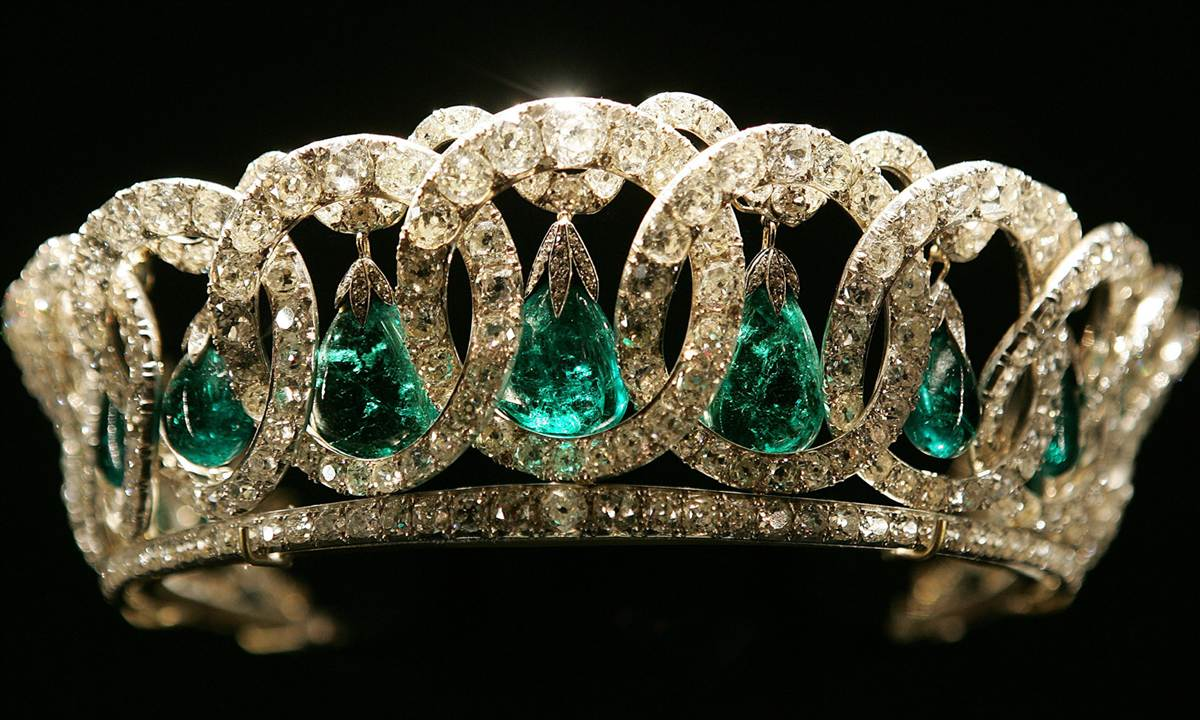
\includegraphics[width=2in]{crown.jpg}
\end{figure}  
}




\end{enumerate}

\problem{We've now proven the CLT, but you may not viscerally feel it yet since all you did is just a bunch of math in bilateral Laplace transform space (which doesn't exactly exalt the spirit). This problem is here to make you really understand the power of this technology. This is a preview to confidence intervals and hypothesis testing which will be the topics of the remainder of this course.}

\begin{enumerate}
%\easysubproblem{Image $X \sim \bernoulli{\half}$. Run the following code in \texttt{R} and print out (in black and white) the result of the following. Does this look like the PMF of $X$? }
%
%\begin{verbatim}
%#first line placeholder
%par(mfrow = c(1, 1))
%N = 10000
%xs = rbinom(N, 1, 0.5)
%h = hist(xs, breaks = 100, plot = FALSE)
%h$counts = h$counts / sum(h$counts)
%plot(h)
%#last line placeholder
%\end{verbatim}
%
%
%\easysubproblem{Now we're going to imagine $X_1, \ldots, X_n \iid \bernoulli{p = 0.5}$ and compute our friend:
%
%\beqn
%C_n = \sqrt{n} \Zbar = \frac{\Xbar - \mu}{\frac{\sigma}{\sqrt{n}}}
%\eeqn
%
%Since we know $\mu = p = 0.5$ and $\sigma = \sqrt{p(1-p)} = \sqrt{0.5 (1 - 0.5)} = 0.5$,
%
%\beqn
%C_n =  \frac{\Xbar - 0.5}{\frac{0.5}{\sqrt{n}}}
%\eeqn
%
%We are going to look at the distribution of $C_n$ for different values of $n$. Remember $C = \limitn C_n$ should be distributed as $\stdnormnot$. Run the following code in \texttt{R} and print out (in black and white) the result (please be patient):
%
%This will look at the estimated PDF for $C_n$ for $n = 10, 100, 1000, 5000, 10000, 50000$. At what $n$ value does it appear that $C_n$ converged to a $\stdnormnot$? Pay attention to gaps of whitespace in these plots. They mean there's no support there! The standard normal has support everywhere. If it never converges, write \qu{never.} }
%
%\begin{verbatim}
%#first line placeholder
%par(mfrow = c(3, 2))
%N = 10000
%mu = 0.5
%sigma = 0.5
%for (n in c(10, 100, 1000, 5000, 10000, 50000)){
%  xs = matrix(rbinom(n * N, 1, mu), ncol = N)
%  xbars = (colMeans(xs) - mu) / (sigma / sqrt(n))
%  hist(xbars, breaks = 100, xlim = c(-4, 4), 
%    main = paste("PDF estimate of Cn for n =", n), col = "blue")
%}
%#last line placeholder
%\end{verbatim}~\spc{1}

\easysubproblem{Now we're going to imagine $X_1, \ldots, X_n \iid \bernoulli{p = 0.1}$ which is more skewed towards failures. Since we know $\mu = p = 0.1$ and $\sigma = \sqrt{p(1-p)} = \sqrt{0.1 (1 - 0.1)} = 0.3$,

\beqn
C_n =  \frac{\Xbar - 0.1}{\frac{0.3}{\sqrt{n}}}
\eeqn

We are going to look at the distribution of $C_n$ for different values of $n$. Remember $C = \limitn C_n$ should be distributed as $\stdnormnot$. Run the following code in \texttt{R} and print out (in black and white) the result (please be patient).

This will look at the estimated PDF for $C_n$ for $n = 10, 100, 1000, 5000, 10000, 50000$. At what $n$ value does it appear that $C_n$ converged to a $\stdnormnot$? Pay attention to gaps of whitespace in these plots. They mean there's no support there! The standard normal has support everywhere. If it never converges, write \qu{never.} }

\begin{verbatim}
#first line placeholder
par(mfrow = c(3, 2))
N = 10000
mu = 0.1
sigma = 0.3
for (n in c(10, 100, 1000, 5000, 10000, 50000)){
  xs = matrix(rbinom(n * N, 1, mu), ncol = N)
  xbars = (colMeans(xs) - mu) / (sigma / sqrt(n))
  hist(xbars, breaks = 100, xlim = c(-4, 4), 
    main = paste("PDF estimate of Cn for n =", n), col = "blue")
}
#last line placeholder
\end{verbatim}
~\spc{2}


\easysubproblem{Now we're going to imagine $X_1, \ldots, X_n \iid \binomial{n = 100}{p = 0.5}$. Since we know $\mu = np = 50$ and $\sigma = \sqrt{np(1-p)} = \sqrt{100 (0.5) (1 - 0.5)} = 5$,

\beqn
C_n =  \frac{\Xbar - 50}{\frac{5}{\sqrt{n}}}
\eeqn

We are going to look at the distribution of $C_n$ for different values of $n$. Remember $C = \limitn C_n$ should be distributed as $\stdnormnot$. Run the following code in \texttt{R} and print out (in black and white) the result (please be patient).

This will look at the estimated PDF for $C_n$ for $n = 10, 100, 1000, 5000$. At what $n$ value does it appear that $C_n$ converged to a $\stdnormnot$? Pay attention to gaps of whitespace in these plots. They mean there's no support there! The standard normal has support everywhere. If it never converges, write \qu{never.} \\ }

\begin{verbatim}
#first line placeholder
par(mfrow = c(2, 2))
N = 10000
mu = 50
sigma = 5
for (n in c(10, 100, 1000, 5000)){
  xs = matrix(rbinom(n * N, 100, 0.5), ncol = N)
  xbars = (colMeans(xs) - mu) / (sigma / sqrt(n))
  hist(xbars, breaks = 100, xlim = c(-4, 4), 
    main = paste("PDF estimate of Cn for n =", n), col = "blue")
}
#last line placeholder
\end{verbatim}~\spc{5}

%\easysubproblem{Now we're going to imagine $X_1, \ldots, X_n \iid \poisson{\lambda = 7}$. Since we know $\mu = \lambda = 7$ and $\sigma = \sqrt{\lambda} = \sqrt{7} = 2.6458$,
%
%\beqn
%C_n =  \frac{\Xbar - 7}{\frac{2.6458}{\sqrt{n}}}
%\eeqn
%
%We are going to look at the distribution of $C_n$ for different values of $n$. Remember $C = \limitn C_n$ should be distributed as $\stdnormnot$. Run the following code in \texttt{R} and print out (in black and white) the result (please be patient).
%
%This will look at the estimated PDF for $C_n$ for $n = 10, 100, 1000, 5000, 10000, 50000$. At what $n$ value does it appear that $C_n$ converged to a $\stdnormnot$? Pay attention to gaps of whitespace in these plots. They mean there's no support there! The standard normal has support everywhere. If it never converges, write \qu{never.} } \pagebreak
%
%\begin{verbatim}
%#first line placeholder
%par(mfrow = c(3, 2))
%N = 10000
%mu = 7
%sigma = 2.6458
%for (n in c(10, 100, 1000, 5000, 10000, 50000)){
%  xs = matrix(rpois(n * N, mu), ncol = N)
%  xbars = (colMeans(xs) - mu) / (sigma / sqrt(n))
%  hist(xbars, breaks = 100, xlim = c(-4, 4), 
%    main = paste("PDF estimate of Cn for n =", n), col = "blue")
%}
%#last line placeholder
%\end{verbatim}~\spc{1}
%
%
%\easysubproblem{Now we're going to imagine $X_1, \ldots, X_n \iid \exponential{\lambda = 7}$. Since we know $\mu = 1 / \lambda = 0.1429$ and $\sigma = 1 / \lambda =  0.1429$,
%
%\beqn
%C_n =  \frac{\Xbar - 0.1429}{\frac{0.1429}{\sqrt{n}}}
%\eeqn
%
%We are going to look at the distribution of $C_n$ for different values of $n$. Remember $C = \limitn C_n$ should be distributed as $\stdnormnot$. Run the following code in \texttt{R} and print out (in black and white) the result (please be patient).
%
%This will look at the estimated PDF for $C_n$ for $n = 10, 100, 1000, 5000$. At what $n$ value does it appear that $C_n$ converged to a $\stdnormnot$? Pay attention to gaps of whitespace in these plots. They mean there's no support there! The standard normal has support everywhere. If it never converges, write \qu{never.} }
%
%\begin{verbatim}
%#first line placeholder
%par(mfrow = c(2, 2))
%N = 10000
%mu = 0.1429
%sigma = 0.1429
%for (n in c(10, 100, 1000, 5000)){
%  xs = matrix(rexp(n * N, 7), ncol = N)
%  xbars = (colMeans(xs) - mu) / (sigma / sqrt(n))
%  hist(xbars, breaks = 100, xlim = c(-4, 4), 
%    main = paste("PDF estimate of Cn for n =", n), col = "blue")
%}
%#last line placeholder
%\end{verbatim}

%\easysubproblem{Now we're going to imagine $X_1, \ldots, X_n \iid \normnot{\mu = 3}{\sigsq = 6^2}$. Since we know $\mu = 3$ and $\sigma = 6$,
%
%\beqn
%C_n =  \frac{\Xbar - 3}{\frac{6}{\sqrt{n}}}
%\eeqn
%
%We are going to look at the distribution of $C_n$ for different values of $n$. Remember $C = \limitn C_n$ should be distributed as $\stdnormnot$. Run the following code in \texttt{R} and print out (in black and white) the result (please be patient).
%
%This will look at the estimated PDF for $C_n$ for $n = 10, 100, 1000, 5000$. At what $n$ value does it appear that $C_n$ converged to a $\stdnormnot$? Pay attention to gaps of whitespace in these plots. They mean there's no support there! The standard normal has support everywhere. If it never converges, write \qu{never.} }
%
%\begin{verbatim}
%#first line placeholder
%par(mfrow = c(2, 2))
%N = 10000
%mu = 3
%sigma = 6
%for (n in c(10, 100, 1000, 5000)){
%  xs = matrix(rnorm(n * N, 3, 6), ncol = N)
%  xbars = (colMeans(xs) - mu) / (sigma / sqrt(n))
%  hist(xbars, breaks = 100, xlim = c(-4, 4), 
%    main = paste("PDF estimate of Cn for n =", n), col = "blue")
%}
%#last line placeholder
%\end{verbatim}~\spc{1}
%
%\intermediatesubproblem{Why did this converge immediately? See question 2(m) for the answer. }\spc{2}
%
%\easysubproblem{Now we're going to get more elaborate. Imagine the following PDF: 
%
%I will consider this to be called the \qu{bathtub function.} This is not a real brand name distribution. I just made it up and it won't be on the test. Write about why you think I called it the \qu{bathtub function.} Does this look like a bell curve at all?? }
%
%\begin{verbatim}
%#first line placeholder
%par(mfrow = c(1, 1))
%N = 10000
%xs = 100 * rbeta(N, 0.1, 0.1)
%h = hist(xs, breaks = 1000, plot = FALSE)
%h$counts = h$counts / sum(h$counts)
%plot(h)
%#last line placeholder
%\end{verbatim}~\spc{2}

\easysubproblem{Now we're going to make sure the central limit theorem works even with stuff that's as crazy as the bathtub. Imagine $X_1, \ldots, X_n \iid \text{bathtub}$. By advanced math, I know $\mu = 50$ and $\sigma = 45.6436$ thus,

\beqn
C_n =  \frac{\Xbar - 50}{\frac{45.6436}{\sqrt{n}}}
\eeqn

We are going to look at the distribution of $C_n$ for different values of $n$. Remember $C = \limitn C_n$ should be distributed as $\stdnormnot$. Run the following code in \texttt{R} and print out (in black and white) the result (please be patient).

This will look at the estimated PDF for $C_n$ for $n = 2, 5, 10, 50, 100, 1000$. At what $n$ value does it appear that $C_n$ converged to a $\stdnormnot$? Pay attention to gaps of whitespace in these plots. They mean there's no support there! The standard normal has support everywhere. If it never converges, write \qu{never.} }

\begin{verbatim}
#first line placeholder
par(mfrow = c(3, 2))
N = 10000
mu = 50
sigma = 45.6436
for (n in c(2, 5, 10, 50, 100, 1000)){
  xs = matrix(100 * rbeta(n * N, 0.1, 0.1), ncol = N)
  xbars = (colMeans(xs) - mu) / (sigma / sqrt(n))
  hist(xbars, breaks = 100, xlim = c(-4, 4), 
    main = paste("PDF estimate of Cn for n =", n), col = "blue")
}
#last line placeholder
\end{verbatim}

\easysubproblem{Let's sum up what we've learned in this problem. The central limit states as $n \rightarrow \infty$ (i.e. it gets big) then $C_n$ becomes a standard normal. Does it become a standard normal at different rates depending on the distribution of the r.v. being sampled? Yes/no is fine.} \spc{2}

\end{enumerate}

\problem{Now that we've now proven the CLT, we are going to use it a little bit. Assume $X_1, \ldots, X_n \iid$ something with mean $\mu$ and standard error $\sigma$.}

\begin{enumerate}

\easysubproblem{Assume $n$ is large enough for the CLT to kick in, show that:

\beqn
\Xbar \sim \normnot{\mu}{\squared{\frac{\sigma}{\sqrt{n}}}}
\eeqn }\spc{1.5}

\easysubproblem{Assume $n$ is large enough for the CLT to kick in, show that:

\beqn
T_n \sim \normnot{n\mu}{\squared{\sqrt{n}\sigma}}
\eeqn }\spc{1.5}


\easysubproblem{Let $X_1, \ldots, X_n \iid \bernoulli{p}$ and let $\Phat := \Xbar$. Assume $n$ is large enough for the CLT to kick in, show that:

\beqn
\Phat \sim \normnot{p}{\squared{\sqrt{\frac{p(1-p))}{n}}}}
\eeqn }\spc{1.5}


\easysubproblem{Draw the PDF of $\Phat_n$ below. On the $\phat$ axis, mark a tick for the mean, and ticks for three standard errors above the mean and ticks for three standard errors below the mean. I'm giving almost a full page for this because other problems depend on it. Use 1/3 of the space for your drawing of the PDF.  }\spc{11}


\hardsubproblem{If $\Xoneton \iid \bernoulli{p}$ and assuming $n$ is big enough for the CLT to \qu{kick in} as well as what you know about normal distributions shifted and scaled, provide the PDF of $\Phat_n$. This will force you to understand (1) the generalized density for $\normnot{\mu}{\sigsq}$ which is in the notes but has never been previously asked on a homework assignment, (2) substitutions for the mean and variance and (3) what the free variable is. }\spc{2}

\intermediatesubproblem{Let's say $p=0.2$ and $n = 100$. What is $\prob{\Phat_n \geq 0.24}$? You will need to use shifts and scales to get it to look like $\prob{Z > z}$ where $Z$ is the standard normal and $z$ is 0.24 standardized.  }\spc{6}

%\hardsubproblem{Let's say $p=0.2$ and $n = 100$. What is the probability of realizing a $\phat$ above 0.3? Without a computer, you cannot answer this exactly. Just using the empirical rule, find the lower and upper bound of this probability. Do not answer exactly. I will not ask you to answer exactly on the test but I will ask you to find a lower and upper bound using the empirical rule.  }\spc{5}

\end{enumerate}

\iftoggle{professormode}{
\paragraph{Basics of Statistical Inference}~\\ \\
} 

\problem{We have now used the CLT to understand the distribution of sample proportions. Here, we will assume that $p$, the true proportion of \qu{success,} is unknown and we will try to infer it. This is a problem of paramount importance. Imagine you're polling for a political candidate. You really do want to know $p$ --- the proportion of people who will vote for your candidate. Imagine you're investigating a drug with side effects. You really do want to know $p$ --- the proportion of people who suffer from that side effect.}

\begin{enumerate}

\easysubproblem{If you have realizations of $\Xoneton \iid \bernoulli{p}$, call them $\xoneton$, what is your best guess of $p$? This is called a \qu{point estimate.} Make sure to use the special notation for this estimate we used in class and define it mathematically.  }\spc{2}

\hardsubproblem{Write \textit{in English} why $\phat \neq p$. I marked this as hard because you need to really use your knowledge about random variables, realizations and parameters and get all these concepts straight.  }\spc{4}

\intermediatesubproblem{Reference the picture in 3(d). Where are the \qu{middle} 95\% of $\phat$'s realized? When I say \qu{middle} I mean the 95\% that are \textit{closest} to $p$, the true expected value. Write the interval that corresponds to this set of numbers. Use the bracket set notation we learned in lecture 1.  }\spc{2}

%\intermediatesubproblem{The interval you created in (c) left out 5\% of the density of $\Phat_n$. Write the set that corresponds to this left out set. Use the union notation from lecture 1.  }\spc{2}

\easysubproblem{What is the width of the interval you created in (c)?  }\spc{0.5}

\easysubproblem{What is the half width of the interval you created in (c)?  }\spc{1}

\easysubproblem{In your picture in 3(d), draw a dotted line from the center of the PDF, $p$ down the length of the page. Create a realization of $\Phat$, call it $\phat$ within the interval in (c) and mark it as a solid dot. Then carefully measure using a ruler, one half width (f) from the fot to the left and one half width from (f) to the right and draw these two lines and mark the ends with a square bracket. No need to write anything below this prompt.}

\easysubproblem{Did this interval \textit{cover} $p$? That is, does it include $p$? You can see if it includes the dotted line drawn down from $p$.  }\spc{1}

\easysubproblem{Would all $\phat$'s realized within the interval in (c) cover $p$?  Yes/no.}\spc{1}

\hardsubproblem{Prove that the probability that the interval covers $p$ is 95\%. We did this in class.  }\spc{4}

\easysubproblem{Illustrate an example of a $\phat$ with the same half-width to the left and right interval that does \textit{not} cover $p$ in your picture of 3(d). No need to write anything here.}

\intermediatesubproblem{In what set do the $\phat$'s such as in (k) come from that fail to cover $p$?  }\spc{1}


\end{enumerate}


\problem{Now we'll just practice building CI's and ask some questions about the procedure.}

\begin{enumerate}

\intermediatesubproblem{Why is it important to have a simple random sample (a completely random sample) when sampling from a population? Write a couple sentences \textit{in English}.  }\spc{4}

\easysubproblem{Write the mathematical definition of a two-sided $1-\alpha$ confidence interval below for a one-sample binomial proportion.  }\spc{1}

\easysubproblem{In the notation above, the \qu{CI} has two subscripts. What do these two subscripts mean?  }\spc{2}

\hardsubproblem{The above CI in (b) does not give \textit{exact} coverage, but only \textit{approximate} coverage for two separate reasons. What are the two reasons? Assume the realizations are indeed sampled from $\iid$ Bernoulli r.v.'s and it was a simple random sample.  }\spc{4}

\easysubproblem{As in the example done in class, imagine we sampled 594 M\&M's and found that 116 were blue. Compute a 95\% CI for $p$, the true proportion of blue M\&M's. Assume all of the CI assumptions are correct.  }\spc{2}

\easysubproblem{Compute a 99\% CI for $p$, the true proportion of blue M\&M's using the same data as in (e). Assume all of the CI assumptions are correct. I gave you this $z_{\overtwo{\alpha}}$ value in class. }\spc{4}

\hardsubproblem{The 99\% CI is larger than the 95\% CI. This is because $z_{\overtwo{\alpha}}$ increased because we requested wider confidence which increases the margin of error (the margin of error is the $z_{\overtwo{\alpha}}\sqrt{\frac{\phat(1-\phat)}{n}}$ term). Let's say we wanted a 99\% CI with the same width as the 95\% CI. How much more M\&M's would we have to look at to do so?  }\spc{6}

\intermediatesubproblem{Let's say we wanted to be sure we captured $p$ in the CI. What's the problem with just making our $1-\alpha$ really large like 99.99999\% (or $\alpha$ really small like 0.000001\%)? Answer \textit{in English}.  }\spc{4}

\easysubproblem{For the interval you created in (e) provide three valid classical interpretations for it \textit{in English}.  }\spc{5}

%\easysubproblem{For the interval you created in (e) write the non-classical i.e subjective interpretation \textit{in English} --- this is the interpretation you really want to be able to say...  }\spc{3}

\easysubproblem{We were interested in political orientation at Queens College. We polled 100 students and 38 of them were registered democrats. Create a 95\% confidence interval for the true proportion of registered democrats at Queens College.  }\spc{4}

\easysubproblem{To get these 100 students, imagine we asked students who were waiting at the Q64 bus stop. Would there then be any problems with the CI we created in (k)? Answer \textit{in English}.  }\spc{3}

\intermediatesubproblem{What would be the best way (or at least a better way) to sample 100 students in order to create the most accurate CI in (k)? Answer \textit{in English}.  }\spc{7}

\end{enumerate}

\problem{CI's are for inference but hypothesis testing is for assessing whether a certain theory is grounded. This will be the last topic covered on the Math 241 final. We will illustrate by using the human sex ratio example from class.}

\begin{enumerate}

\easysubproblem{We a priori assume an equal sex ratio. We'll define $p$ as the probability of being male arbitrarily. What is the null hypothesis expressed using the mathematical notation we used in class? }\spc{1}

\easysubproblem{What would be the alternative hypothesis expressed using the mathematical notation we used in class? }\spc{1}

\intermediatesubproblem{If $n=200$, what is the null distribution? No symbols are acceptable as an answer, you must calculate exactly what the distribution is. Draw this null distribution how we did in class. }\spc{6}

\intermediatesubproblem{Let's say failing to find a deviation from the hypothesized equal sex ratio meant you get fired from your boss (who believes in the unequal sex ratio theory). What kind of $\alpha$ would you pick for this test? Justify using a sentence \textit{in English}. }\spc{3}

\easysubproblem{Regardless of the $\alpha$ chosen, choose $\alpha = 1\%$. What is the retainment region under $\alpha = 1\%$? Denote it on the drawing in (c). }\spc{2}

\easysubproblem{What is the rejection region under $\alpha = 1\%$? Use the $\cup$ symbol to join the two sets. Denote it on the drawing in (c). }\spc{2}

\easysubproblem{What is a Type I error in general? Answer \textit{in English}. }\spc{3}

\easysubproblem{What does a Type I error mean in this human sex ratio experiment? Answer \textit{in English}. }\spc{3}

\easysubproblem{What is the probability of the Type I error in this example? }\spc{1} 

\easysubproblem{What is a Type II error in general? Answer \textit{in English}. }\spc{3}

\easysubproblem{What does a Type II error mean in this human sex ratio experiment? Answer \textit{in English}. }\spc{3}

\easysubproblem{You count there are 113 males. Calculate $\phat$ and denote it on the drawing in (c).  }\spc{3}

\easysubproblem{What is the result of the hypothesis test? Do you retain $H_0$ or reject $H_0$? Write a sentence in English interpreting what this means.  }\spc{4}

\hardsubproblem{Now let $n=4,247,000$ (the number of American newborns in the year 2008) and use the same $\alpha =1\%$. You get 2,173,000 males. Write the hypotheses, find the retainment region and find the result and interpret it. }\spc{9}

%\extracreditsubproblem{Why is the human sex ratio not even? Write your thoughts below with sources. }\spc{5}

\end{enumerate}

\problem{This last example involved two-sided hypothesis tests of one proportion. Here, we will examine the case of firing the Uber driver where we only care about only testing one side.

The Uber driver takes 1,000 rides and then the company makes a decision about whether or not he's a good driver based on an arbitrary rule of having more than $p=$ 5\% true proportion / propensity of bad rides.}

\begin{enumerate}

\easysubproblem{Detecting him being a bad driver is sounding the alarm. Thus the status quo is that he's a good driver. Thus, $H_0: p \leq 0.05$. What is $H_a$ here?  }\spc{1}

\intermediatesubproblem{At $\alpha$ = 2.5\%, what is the retainment region? }\spc{2}

\easysubproblem{At $\alpha$ = 2.5\%, what is the rejection region? }\spc{2}

\easysubproblem{The driver under investigation had 62 badly reviewed rides out of 1,000 rides. Calculate $\phat$ and say if it's above the $p$ cutoff Uber is using. }\spc{1}

\intermediatesubproblem{If the driver under investigation had 62 badly reviewed rides out of 1,000 rides, would Uber fire him? Run the hypothesis test now and see. Hint: the answer to the (d) will mislead you. }\spc{8}

%\hardsubproblem{You may be wondering why on Earth we defined $H_a$ the way we did in (a). Wouldn't it seem more natural to switch the null and alternative hypothesis? Switch them here and run the test again. }\spc{6}
%
%\hardsubproblem{Your answer changed! Why is it a bad idea to run the test like in (f) / why is it a better idea to run the test like in (e)? }\spc{4.5}


\extracreditsubproblem{Find the $p$-val for the test in (e). }\spc{0}

\extracreditsubproblem{If the driver's true proportion / propensity of bad rides is $6\%$, what is the probability of a type II error when running the test in (e)? Then calculate power (1 - the probability of a type II error).}\spc{0}

\end{enumerate}

\problem{This will teach you about $H_0$ and $H_a$ using a silly example. This problem is optional and will not be graded.}

\iftoggle{professormode}{
\begin{figure}[htp]
\centering

\includegraphics[width=2in]{ufo.jpg}
\end{figure}  
} 

\begin{enumerate}

\easysubproblem{Consider $H_0$: Aliens do not exist vs $H_a$: Aliens do exist. Why is this a \qu{standard} hypothesis test? [optional] }\spc{1}

\easysubproblem{Describe a person using English who has a high $\alpha$ for $H_0$: Aliens do not exist vs $H_a$: Aliens do exist. [optional] }\spc{1}

\easysubproblem{Describe a person using English who has a low $\alpha$ for $H_0$: Aliens do not exist vs $H_a$: Aliens do exist. [optional] }\spc{1}

\easysubproblem{Describe a person using English who has a high $\alpha$ for $H_0$: Aliens do exist vs $H_a$: Aliens do not exist. [optional] }\spc{1}

\easysubproblem{Describe a person using English who has a low $\alpha$ for $H_0$: Aliens do exist vs $H_a$: Aliens do not exist. [optional] }\spc{2}

\end{enumerate}

\end{document}
